\documentclass{article}
\usepackage[utf8]{inputenc}
\usepackage{amsmath}
\everymath{\displaystyle} % better layout

\usepackage{hyperref} % hyperlinks 
\usepackage{xcolor} % colors
\usepackage{graphicx} % figures

\usepackage[margin=1.3in]{geometry} % smaller margins 



% some math commands
\newcommand{\de}[0]{\mathrm{d}}
\newcommand{\dx}[0]{\de x}
\newcommand{\dt}[0]{\de t}
\newcommand{\ds}[0]{\de s}
\newcommand{\dpartial}[2]{\frac{\partial #1}{\partial #2}}
\newcommand{\dtotal}[2]{\frac{\de #1}{\de #2}}

% a big "to do" signal
\newcommand{\todo}[0]{\colorbox{yellow}{\textcolor{red}{TODO}}}



\setcounter{tocdepth}{4}

\begin{document}

\tableofcontents

\newpage

\section{Foglio 1}
\subsection{1 - Osservatori uniformemente accelerati}
Considero una particella $P_0$, uniformemente accelerata rispetto al sistema istantaneamente inerziale  $\mathcal{I}$.
Il sistema $\mathcal{I}$ va inteso come un insieme di sistemi di riferimento inerziali, tra i quali, per ogni tempo, si considera quello rispetto a cui la particella $P_0$ \`e istantaneamente ferma.
\paragraph{Particella accelerata}
Considero una generica particella $P$, con velocit\`a $u$ e accelerazione $a$ nel sistema $\mathcal{I}$
Scrivo il boost a velocit\`a inversa dal sistema in movimento $\mathcal{I}$ al sistema terra $\mathcal{T}$:
\begin{equation}
	\begin{cases}
		\dx_T = \gamma (\dx + v \dt) &  \\
		\dt_T = \gamma (\dt + v \dt) &  \\ 
	\end{cases}
\end{equation}
\[  u_T = \frac{\dx_T}{\dt_T} = \frac{u+v}{1+uv} \]
\[ \de u_T = \frac{1-v^2}{(1+uv)^2} \de u \]
\begin{equation} \label{accel_P}
	a_T = \frac{\de u_T}{\dt} = \frac{(1-v^2)^{3/2}}{(1+uv)^3} a 
\end{equation}
Volendo trovare la velocit\`a della particella $P_0$, utilizzo l'equazione \ref{accel_P} e la specializzo: la velocit\`a $u$ va posta nulla perch\`e considero la particella $P_0$, ferma in $\mathcal{I}$, e considero l'evoluzione temporale di $v(t_T)$, rispetto al sistema $\mathcal{T}$; la velocit\`a della particella rispetto a $\mathcal{T}$ \`e adesso $v$ e \( a = a_0 \):
\[ a_T = \frac{\de v(t_T)}{\dt_T} = [1-v^2(t_T)]^{3/2} a_0 \]
\[ a_0t_T = \int_0^{v(t_T)} \frac{\de v}{(1-v^2)^{3/2}} \]
sostituisco $v=\sin(\theta)$
\[ a_0t_T= \int_0^{\arcsin(v(t_T))} \frac{\de \theta}{\cos^2(\theta)} = \int \de\tan\theta = \tan(\arcsin(v(t_T))) \]
\[ v(t_T) = \sin(\arctan(a_0t_T)) \]
\begin{equation} \label{veloc}
		v(t_T) = \frac{a_0 t_T}{\sqrt{1+(a_0t_T)^2}} 
\end{equation}

Per trovare la legge oraria, considerando che \(x_T(0)=v_T(0)=0\),
\[ \int_{x_T(0)}^{x_T(t_T)} \dx_T = \int_0^{t_T} \frac{a_0t_T}{\sqrt{a+(a_0t_T)^2}} \dt_T \]
Sostituendo prima \( y=a_0t_T \) e poi \( y = \sinh(z) \) si ottiene
\[ x_T(t_T) = \frac{1}{a_0} \int_{y_0}^y \frac{y}{\sqrt{1+y^2}} \de y \]
\[ = \frac{1}{a_0} \int_{z_0}^z \sinh(z) \de z \]	
\[ = \frac{1}{a_0} [\cosh\sinh^{-1}(y) - \cosh\sinh^{-1}(y_0)] \]
\[ = \frac{1}{a_0} [\cosh(\ln(y + \sqrt{1+y^2}) -1] \]
\[ = \frac{y^2+y\sqrt{1+y^2}+1-y-\sqrt{1+y^2}}{a_0(y+\sqrt{1+y^2})} \]
\[ = \frac{\sqrt{1+y^2}-1}{a_0} \]
\begin{equation} \label{leggeoraria}
	x_T(t_T) = \frac{\sqrt{1+(a_0t_T)^2}-1}{a_0} 
\end{equation}
\todo limite di basse velocit\`a

\paragraph {Achille e la lepre}
Uguagliando c*t a xT dovrei trovare qualcosa, ma se metto c=1 si cancella tquadro e se lo tengo non so dove sbattere la testa.

\paragraph {Tempo proprio}
Con \(\de s^2 = -c^2\dt^2 + \dx^2 \):
\[ ic\de\tau = \de s = ic\dt_T \sqrt(1*-v^2(t_T)) \]
\[ \tau = \int_0^{t_T} \sqrt(1*-v^2(t)) \dt = \int \frac{1}{\sqrt{1+(a_0t)^2}} \dt \]
Sostituendo \( a_0t = \cosh z \)
\[ \tau = \int \frac {\de z}{a_0} = \frac{\sinh^{-1}(a_0t_T)}{a_0} = \frac{\ln({\sqrt{1+(a_0t_T)^2}+a_0t_T)}}{a_0}\]

\paragraph {$10^9$ anni-luce} \todo udm di c
Per percorrere una distanza di $10^9 \mathrm{ly}$ con accelerazione da fermo di \(g=9.8m/s^2=1.030ly/y^2\), usando la formula \ref{leggeoraria}, occorrono
\[ \sqrt{\frac{d}{c}^2 + 2\frac{d}{g}} \simeq 2.998\cdot10^18y \]
cui corrisponde un tempo proprio \( \tau \simeq 41.972 y \).

\paragraph {Perch\`e non andiamo su Giove?}
Con le formule della meccanica classica,
\[ t_{TOT} = 4\cdot \sqrt{\frac{2x_{TM}}{g}} = 2.8558587119250753 y \]
In relativit\`a ristretta, dove 'lh' sono le ore-luce,
\[ t_{TM} = 260.627804384274lh \]
\[ v_{TM} = 0.9999999999999941 c \]
Modificando opportunamente la formula \ref{veloc} per velocit\`a iniziale non nulla, si ottiene
\[ v(t_T) = \frac{a_0 t_T + \tan\arcsin(v_0)          }
	{\sqrt{1+( a_0t_T + \tan\arcsin(v_0)           )^2 }}  \]
\[ v(t_T) = \frac{a_0 t_T + \frac{v_0}{\sqrt{1-v_0^2}} }
	{\sqrt{1+( a_0t_T + \frac{v_0}{\sqrt{1-v_0^2}}  )^2 }}  \]
E per la legge oraria
\[ x_T(t_T) = \frac{\sqrt{1+ (-gt_T + \frac{v_0}{\sqrt{1-v_0^2}})^2 } - 
	\sqrt{1+  (\frac{v_0}{\sqrt{1-v_0^2}})^2}     }{-g} \]
Invertendo:
\[ t = \frac{ \frac{v_0}{\sqrt{1-v_0^2}} + \sqrt{ (\frac{v_0}{\sqrt{1-v_0^2}})^2 - 2gx \sqrt{1+( \frac{v_0}{\sqrt{1-v_0^2}}    )^2     }  } }
             {  g   }\]
\todo risultati bruttissimi

2.99792458e+18  anni
tempo proprio:
41.9715540832882 anni




\paragraph{Razzo relativistico}
Considero il sistema $\mathcal{I}$ in cui il razzo \`e fermo e i sistemi $\mathcal{E}$, in cui \`e ferma la $\de m$ espulsa, e $\mathcal{J}$, in cui \`e fermo il razzo propulso con massa $m-\de m$. Nel sistema $\mathcal{I}$:
\[ \de m v_e \gamma(v_e) = (m - \de m) \de v \gamma(\de v) \sim m \de v \]
\[ \frac{\de m}{m} = \frac{1}{v_e \gamma(v_E)} \frac{\de v}{\de\tau} \de\tau \]
\[ m = m_0 e^{\frac{\frac{\de v}{\de\tau}}{v_e \gamma(v_e) }} \]
\[ m = m_0 e^{\frac{a_0\tau}{v_e \gamma(v_e) }} \]

\paragraph{Campo elettrico}













































\section{Foglio 2}
\subsection{Proiezione stereografica}
Per un cerchio, valgono le relazioni seguenti:
\[ x_{N,S} = R \frac{\sin\theta}{1\mp\cos\theta} \]
Nel caso di una sfera, in coordinate polari tale relazione varra' per il modulo rispetto alla latitudine; la longitudine dara' invece l'argomento. Riscrivendo in campo complesso:
\[ z_{N,S} = \rho_{N,S} e^{i\varphi} \]
\[ \bar{z}_{N,S} = \rho_{N,S} e^{-i\varphi} \]
con 
\[ \begin{cases}
	\rho_{N,S} = R \frac{\sin\theta}{1\mp\cos\theta} & \\
	\varphi_{N,S} = \phi & \\
   \end{cases}
\]


Si definisce la funzione che lega le due carte nel modo seguente:
\[ z_N = \frac{1}{z_S} \]
\[ \bar{z}_N = \frac{1}{\bar{z}_S} \]
Tale relazione \`e olomorfa in \( U_N \cap U_S \), cio\`e il piano complesso senza l'origine e l'infinito.
Le coordinate $w_{N,S}$, ottenute proiettando sul piano tangente alla sfera nel polo opposto, hanno modulo doppio delle rispettive $z_{N,S}$:
\[ w_{N,S} = 2z_{N,S} \]

\subsection{Rotazioni}
I calcoli di questo paragrafo si intendono fatti con $z_N$. % Le derivate si considerano per ora applicate a funzioni olomorfe.
\[ L_z = -i\dpartial{}{\phi} = -i \dpartial{\varphi}{\phi}(\dpartial{z}{\varphi}\dpartial{}{z} + \dpartial{\bar{z}}{\varphi}\dpartial{}{\bar{z}}) = z\dpartial{}{z} - \bar{z}\dpartial{}{\bar{z}}\]
\[ L_\pm = \pm e^{\pm i\phi} (\dpartial{}{\theta} \pm i \cot\theta \dpartial{}{\phi} ) \]
\[ = \pm e^{\pm i\varphi}Re^{i\varphi}  (-\frac{1}{1- \cos\theta} \mp  \cot\theta \frac{\sin\theta}{1-\cos\theta})\dpartial{}{z} \pm e^{\pm i\varphi}Re^{-i\varphi}  (-\frac{1}{1- \cos\theta} \pm  \cot\theta \frac{\sin\theta}{1-\cos\theta})\dpartial{}{\bar{z}} \]

Siccome \( z\bar{z} = \frac{1+c}{1-c}\),
\[ L_+ = -\frac{z^2}{R}\dpartial{}{z} -R\dpartial{}{\bar{z}} , \;\;\;\;\;\;  L_- = R\dpartial{}{z} + \frac{\bar{z}^2}{R}\dpartial{}{\bar{z}} \]
Usando che \( \frac{\partial^2}{\partial z \partial \bar{z}} = \frac{\partial^2}{\partial \bar{z} \partial z}\) 
\[ [L_+,L_-] = 2L_z \]



\subsubsection*{Autovalori di $F_m$}
Tenendo conto che 
\[ L_z f(\rho) = (z\dpartial{\rho}{z} - \bar{z}\dpartial{\rho}{\bar{z}}) \dpartial{f}{\rho} = 0\]
\`e immediato verificare che 
\[ L_z F_m = L_z[z^m] f(\rho) + z^m L_z[f(\rho)] = m F_m\]


\subsubsection*{Forma di $Y_l^l$}
\[ L_+ [f(z\bar{z})] = (-z^2\dpartial{\rho}{z} - \dpartial{\rho}{\bar{z}} ) \dpartial{f}{\rho} \]
\[ = -\frac{z^{m+1}}{R} \left[ mf + (|z|^2+R^2) \dpartial{f}{\rho^2}   \right] \]
Imponendo l'annullamento della parentesi si trova un'equazione differenziale che ha soluzione
\[ f_m (\rho^2) = f_m(\rho^2 + R^2)^{-m} \]
Definendo 
\[ Y_l^m = z^m f_m(\rho^2 + R^2)^{-m}  \]
si vede infine che 
\[ L_+Y^m_l = 0 \iff m=l \]
\[ L_-Y_l^l = (\frac{mR}{z} +\frac{\bar{z}}{R}) Y_l^l \]

Nelle coordinate $(z_S, \bar{z}_S)$
\[ Y_l^m = z_S^{-m}f_m((z_S\bar{z}_S)^{-1} + R^2)^{-m}  \]




\section{Foglio 3}
\subsection{Metrica bidimensionale}
Si studia la metrica
\[ g = \de s^2 = \frac{\epsilon \de x^2 + \de y^2}{y^2} \]
con \( \epsilon = \pm 1\).

\subsubsection*{Vettore di Killing} \todo
Considerando che la metrica non dipende dal modulo di x, ma solo da quello di y, si scrive immediatamente che per 
\[ \vec{k} = \left( \begin{array}{c}  cost \\ 0 \end{array}  \right) \]
\[ \mathcal{L}_{\vec{k}} g = 0 \]

\subsubsection*{Simboli di Christoffel}
L'azione di una particella libera, in parametrizzazione affine, si scrive
\[ S = \frac{1}{2} \int \de \lambda \frac{\epsilon \dot{x}^2 + \dot{y}^2}{y^2} \]
Le variazioni $\delta x$ portano a 
\[ \left(\frac{\epsilon \dot{x}}{y^2}\right)^\cdot = 0 \]
\[ \ddot{x} - \frac{2\dot{x}\dot{y}}{y} = 0 \]
mentre per $\delta y$ si ha
\[ \frac{\epsilon \dot{x}^2 + \dot{y}^2}{y^3} + \left(\frac{\dot{y}}{y^2}\right)^\cdot =0 \]
\[ \ddot{y} + \left(\frac{\epsilon \dot{x}}{y} - \frac{\dot{y}^2}{y} \right) =0 \]
Confrontando le'equazioni con la condizione per le geodetiche
\[ \ddot{x}^\mu + \Gamma^\mu_{\sigma\rho} \dot{x}^\sigma\dot{x}^\rho =0 \]
si trovano
\[ \Gamma^x_{xy} = \Gamma^x_{yx} = -\frac{1}{y} ; \;\;\; \Gamma^y_{xx} = \frac{\epsilon}{y} ; \;\;\; \Gamma^y_{yy} = - \frac{1}{y} \]
Ovvero
\begin{equation}
	\begin{pmatrix}
		\Gamma^x_{\; x} & \Gamma^x_{\; y} \\
		\Gamma^y_{\; x} & \Gamma^y_{\; y} 
	\end{pmatrix} = 
	\begin{pmatrix}
		-\frac{\de y}{y} 	& -\frac{\de x}{y}  \\
		\frac{\epsilon\de x}{y} & -\frac{\de y}{y} 
	\end{pmatrix}
\end{equation}
Con i simboli cos\`i trovati, si possono scrivere le seguenti equazioni
\begin{equation} 
	\begin{cases}
		\nabla e_x = -\frac{\de y}{y} \otimes e_x + \frac{e \de x}{y} \otimes e_y & \\ 
		\nabla e_y = -\frac{\de x}{y} \otimes e_x - \frac{\de y}{y} \otimes e_y & \\
	\end{cases}
\end{equation}

\subsubsection*{Tensore curvatura}
\[ R = \de\Gamma + \Gamma\wedge\Gamma \]
\begin{equation}
	(\de\Gamma)^i_j = \partial_\rho \Gamma_{\mu j}^i \dx^\rho \dx^\mu = \partial_y 
		\begin{pmatrix}
			0 & \frac{1}{y} \\
			-\frac{\epsilon}{y} & 0 \\
		\end{pmatrix}
		\dx\wedge\de y
\end{equation}
\[ (\Gamma\wedge\Gamma)^i_j = \Gamma^i_j\wedge\Gamma^j_k \]
e utilizzando il fatto che 
\[ \dx^\mu\wedge\dx^\mu = 0 = \dx^\mu\wedge\dx^\nu + \dx^\nu\wedge\dx^\mu \]
si trova che \( \Gamma\wedge\Gamma = 0 \).
Ne segue che 
\[ R = \frac{1}{y^2} 
	\begin{pmatrix}
		0 & -1 \\
		\epsilon & 0 \\
	\end{pmatrix}
	\dx\wedge\de y
\]
Il tensore di Ricci \`e 
\[ \mathrm{Ric}_{j\nu} = \delta^\mu_i R^i_{j\mu\nu} \]
E come matrice
\[ \mathrm{Ric} = 
	\begin{pmatrix}
		-\frac{\epsilon}{y^2} & 0 \\
		0                     & -\frac{1}{y^2} \\
	\end{pmatrix}
\]
Lo scalare di curvatura \`e definito come 
\[ R = g^{ij} R_{ij} \]
Si calcola $g^{ij}$ come inverso della metrica, da cui
\[ ||g^{ij}|| = \mathrm{diag}(\frac{y^2}{\epsilon}, y^2) \]
e $R=-2$.

\subsubsection*{Zweibein}
Scrivendo
\[ V^x = \frac{\dx}{y} \;\;\;\;\; V^y = \frac{\de y}{y} \;\;\;\;\; \eta_{ij} = 
	\begin{pmatrix}
		\epsilon & 0 \\
		0        & 1 \\
	\end{pmatrix}
\]
si ha
\[ \de s^2 = \eta_{ij} V^iV^j \]
\newline
Sapendo che 
\[ 	\begin{cases}
	\de V^x = \partial_y \left(\frac{1}{y}\right) \de y \wedge \dx & \\
	\de V^y = \partial_x \left(\frac{1}{y}\right) \dx \wedge \de y = 0  & \\
	\end{cases}
\]
e, considerando \(T^i = 0\), 
\[ \de V^i = -\omega^i_j\wedge V^j \]
(gli indici sono ora intesi nello spazio delle zweibein)
si trova
\[ \omega^y_x \wedge V^x = 0 \]
\[ \omega^x_y \wedge V^y = \frac{1}{y^2} \de y \wedge \dx \]
Considerando che, con la metrica piatta,
\[ V_i = \eta_{ij} V^j = \begin{cases}
	\epsilon V^i & \mathrm{se} \;\; i=x \\
	V^i	     & \mathrm{se} \;\; i=y \\
\end{cases} \]
si trova che 
\[ \omega^x_y \wedge V^y = -V^x\wedge V^y \]
da cui 
\[ \omega^x_y = -V^x \]
e naturalmente
\[ \omega^y_{\,x}= \epsilon\omega^{yx} = -\epsilon\omega^{xy} = -\epsilon\omega^x_{\,y} \]
che verifica la condizione trovata per $\de V^y$.
L'antisimmetria di $\omega^i_{\;j}$ si trasferisce a $R^i_{\;j}$, che avr\`a non nulli solo
\[ R^x_{\;y} = \de \omega^i_{\;j} = -V^x\wedge V^y \;\;\;\;\; R^y_{\;x} = -\epsilon\de \omega^i_{\;j} = \epsilon V^x\wedge V^y \]
Pertanto 
\[ R = \begin{pmatrix}
		0 & -1 \\
		\epsilon & 0 \\
	\end{pmatrix} V^x \wedge V^y \]
Il tensore di Ricci ha componenti
\[ \mathrm{Ric}_{ij} = 
	\begin{pmatrix}
		R^y_{x|yx} & R^x_{x|xy} \\
		R^y_{y|yx} & R^x_{y|xy} \\
	\end{pmatrix}
	= \begin{pmatrix}
		R^x_{\;y} & 0 \\
		0 & R^x_{\;y} \\
	\end{pmatrix}
	= \begin{pmatrix}
		-\epsilon & 0 \\
		0 & -1 \\
	\end{pmatrix}
\]
per cui lo scalare 
\[ R = g^{ij} \mathrm{Ric}_{ij} = -\epsilon^2 -1=-2 \]

\subsubsection*{Derivate covarianti}
I vettori tangenti alle Zweibein sono quelli tali per cui
\[ e_i(V^j) = \delta_i^j \]
e sono pertanto
\[ e_x = y \dx \;\;\;\;\; e_Y = y\de y \]
Se ne calcolano le derivate covarianti, con connessione $\omega^i_{\;j}$:
\[ \nabla e_x = \omega^y_{\;x} e_y = \epsilon e_y \otimes V^x \;\;\;\;\; \nabla e_y = \omega^x_{\;y} e_x =  e_x \otimes V^x \]



\subsubsection*{Integrali primi}
Gli integrali primi
\[ \begin{cases}
	p_x = \frac{\dot{x}}{y^2} & \\
	\sigma = \frac{\epsilon\dot{x}^2 + \dot{y}^2}{y^2} & \\
  \end{cases}
\]
danno le condizioni
\[ \begin{cases}
	\dot{x} = p_x y^2 & \\
	\dot{y}^2 = (\sigma - \epsilon p_x^2 y^2 ) y^2 & \\
  \end{cases}
\]
Si procede calcolando
\[ \left(\frac{\de v}{\dx}\right)^2 = \left( \frac{\de v}{\de \lambda} \frac{\de \lambda}{\dx}  \right)^2 
	= \left( \frac{2\dot{y}y}{\dot{x}} \right)^2 \]
e, sostituendo le condizioni trovate con gli integrali primi, si ottiene
\[ \left(\frac{\de v}{\dx}\right)^2 = \frac{4}{p_x^2} (\sigma - \epsilon\dot{x}^2 y^2 )\]

Per integrare questa equazione,
\[ \frac{\de v}{\dx} = \frac{2}{p_x}\sqrt{\sigma - \epsilon p_x^2 v} \;\;\; \Rightarrow \;\;\;
	\frac{2\sqrt{\sigma}}{p_x} \dx = \frac{\de v}{ \sqrt{1 - \frac{\epsilon p_x^2 v}{\sigma}}} \]
Si sostituisce al secondo membro 
\[ v \rightarrow q = \frac{\epsilon p_x^2 v}{\sigma} \;\;\;\Rightarrow\;\;\; 
	\frac{\sigma}{\epsilon p_x^2} \frac{\de q}{\sqrt{1-q}} \]
Un'ulteriore sostituzione porta a 
\[ q \rightarrow \theta=\arcsin{\sqrt{q}} \;\;\;\Rightarrow\;\;\;
	\frac{2\sigma}{\epsilon p_x^2} \de{\cos\theta} \]
Pertanto, tenendo conto che 
\[ \cos\arcsin\sqrt{q} = \sqrt{1-q} \]
l'integrazione porta a 
\[ \frac{p_x\epsilon}{\sqrt{\sigma}}(x-x_0) = \sqrt{1-\frac{\epsilon p_x^2 v}{\sigma}} -c_0 \]
che raccogliendo le costanti e riarrangiando porta a 
\[ (p_x \epsilon x - K)^2 = \sigma - \epsilon p_x^2v \]
Al variare di $\epsilon$ e $\sigma$, si ottengono i seguenti grafici:
\begin{figure}[htbp]
 \centering
 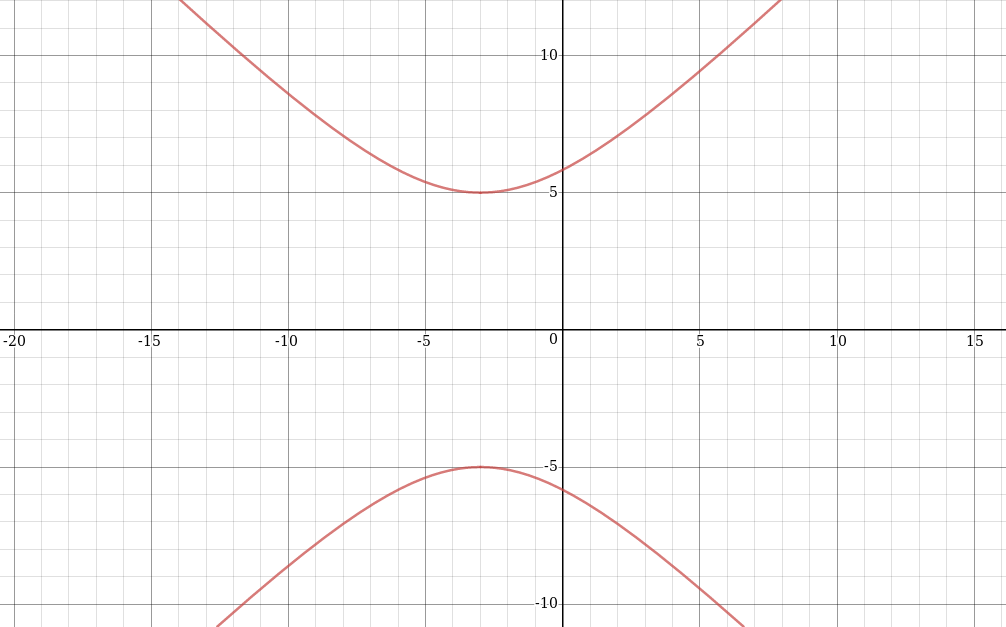
\includegraphics[width=\textwidth]{images/foglio3_neg_neg}
	\caption{\(\epsilon=-1, \;\sigma=-1\)}
 \label{figure:neg_neg}
\end{figure}
\begin{figure}[htbp]
 \centering
 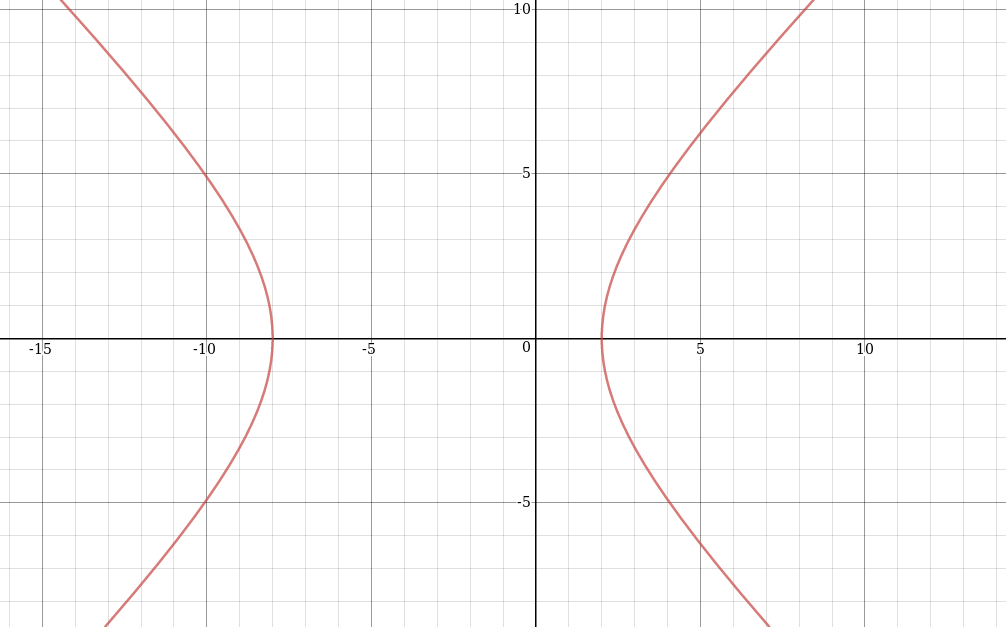
\includegraphics[width=\textwidth]{images/foglio3_pos_neg}
	\caption{\(\epsilon=-1, \;\sigma=+1\)}
 \label{figure:pos_neg}
\end{figure}
\begin{figure}[htbp]
 \centering
 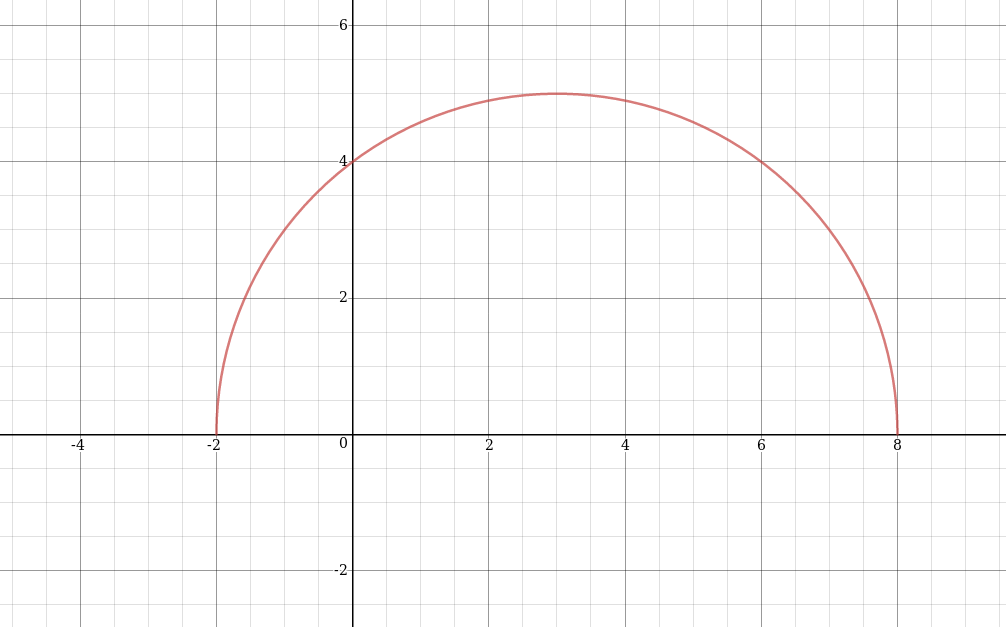
\includegraphics[width=\textwidth]{images/foglio3_pos_pos}
	\caption{\(\epsilon=+1, \;\sigma=+1\)}
 \label{figure:pos_pos}
\end{figure}





















\end{document}
